%Project Narrative
\documentclass[12pt]{article}
\usepackage[margin=1.1in]{geometry}
\usepackage{color}
\usepackage{graphicx}
\usepackage{url}
\usepackage{multicol}
\usepackage{wrapfig}
\usepackage{amsmath}
\usepackage{amssymb}
\usepackage{caption}
\usepackage{subcaption}
\usepackage[round]{natbib}
\bibliographystyle{evolution}
\usepackage[usenames,dvipsnames,svgnames,table]{xcolor}
\usepackage[innercaption]{sidecap} % side captions
\sidecaptionvpos{figure}{c}

\newcommand{\jri}[1]{\textcolor{blue}{ \emph{\scriptsize  #1}} }
\newcommand{\kc}[1]{\textcolor{violet}{ \emph{\scriptsize  #1}} }
\newcommand{\citex}{\textcolor{red}{\textbf{(CITE)}}}

\begin{document}

\title{\vspace{-5ex}The genetic archaeology of maize: reconstructing pedigrees to identify useful diversity for breeding\vspace{-4ex}}
\author{}
\date{}
\maketitle

\section*{Rationale and Significance}
\label{sec:rationale}

Maize is a natural resource of fundamental national importance, vital for food, livestock feed, and fuel production.
Maize is also the most valuable field crop in the United States, with production values at greater than \$50 billion dollars every year since 2010 \citep{usdanass}. 

But while maize yields have increased over the last several decades, the rate of gain falls short of projected needs in the near future \citep{grassini2013distinguishing}.
Even under stable climatic conditions, current rates of maize improvement are insufficient to meet requirements of population growth over the next 30 years \citep{ray2013yield}; in  addition to requirements in terms of food and animal feed, worldwide ethanol use is projected to increase 40\% within just the next decade \citep{usdalong}.
%could be convinced to drop the ethanol comment

Changing climatic conditions, however, will likely further challenge our ability to meet needed yield gains. 
Historical analyses suggests that climate change over the last 30 years has already dramatically impacted maize yields worldwide, retarding gains from breeding and management \citep{Lobell2011}.
Moreover, predicted temperature increases will increase volatility in yield across the U.S. and may even decrease future yields \citep{urban2012projected}, with some models suggesting a change of even 1$^{\circ}$C could negatively impact yields by as much as 17\% \citep{lobell2003climate}; more dire warnings suggest that U.S. maize yields could drop 30-46\% below current levels by the end of the century \citep{schlenker2009nonlinear}.
Substantial efforts will clearly be needed to preserve U.S. maize production and increase or maintain yields.  

Much of the historical gains in maize yield can be directly attributed to breeding efforts \citep{Duvick1992, duvick2005genetic}, and \textbf{ breeding must remain of central importance in order to meet increased yield demands}.  
Breeding is also of key importance in adapting maize to the challenges of changing climates \citep{Troyer2004a}, with recent models suggesting that efficient use of extant adaptive diversity in maize could significantly ameliorate the effects of climate change \citep{butler2013adaptation}.   

\subsection*{Diversity loss threatens breeding gains}

Breeding, and adaptation in general, relies critically on the availability of genetic diversity. 
This is best represented mathematically by JL Lush's famous ``breeder's equation'':

\begin{align}
R=\frac{V_A}{V_P}s
\label{eq:lush}
\end{align}

showing that adaptation --- the response to selection $R$ --- depends not only on the strength of selection $s$ but also directly on the amount of heritable genetic variation $V_A$ for the trait of interest \citep{kelly2011breeder}. 
The advent of modern hybrid maize breeding, the development of distinct breeding pools and the winnowing of inbreds from individual breeding programs has led to a marked decrease in genetic diversity. 
Analyzing genotypes of more than 4000 public and recently released private lines, we recently showed that the diversity available to maize breeders in current germplasm is less than half what it was in before 1950 (Figure \ref{fig:diversity}). 
With decreasing diversity available for breeding decreasing yield gains are a mathematical certainty. 
%over the top?

\begin{SCfigure}
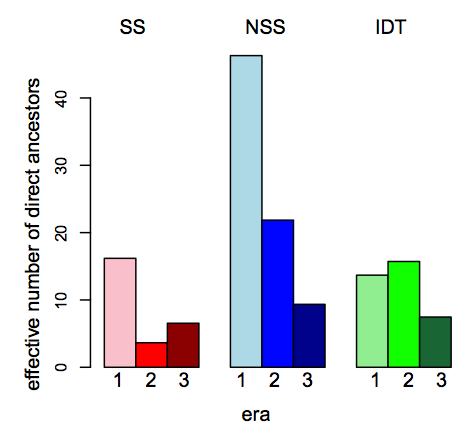
\includegraphics[width=0.5\linewidth]{joost_diversity.png}
\caption{Changes in genetic diversity (represented as the effective number of ancestors) of the three primary maize heterotic groups (SS: stiff-stalk; NSS: non-stiff-stalk; IDT: iodent). Inbreds are divided into eras representing different time periods: 1:1930-1950; 2:1950-1980; 3:1985-1992. Figure from \citet{van2012historical}.} 
\label{fig:diversity}
\end{SCfigure}

While open-pollinated varieties and exotic inbred lines represent a viable source of new diversity, these have been only sparingly used in the private sector due to their poor agronomic performance, photoperiod sensitivity, and the necessary generations of back-crossing to adapted lines required to incorporate useful alleles into high-performing temperate germplasm \citep{goodman1999broadening}.
In contrast, older U.S. inbred lines, though lower-yielding than their contemporaries, harbor novel genetic diversity of potential use for breeding but are already adapted to the U.S. cornbelt.  
Breeders have clearly bee successful in advancing high-yielding germplasm and discarding ill-adapted material.
This does not mean, however, that all discarded material has little genetic merit --- beneficial alleles can be lost to genetic drift, particularly considering the polygenicity of agronomic traits and also because breeders are unable to select for all traits simultaneously. Our own population genetic analysis supports this notion; a number of underutilized older inbreds are enriched with favorable alleles (Figure \ref{fig:wf9}). 

\begin{SCfigure}
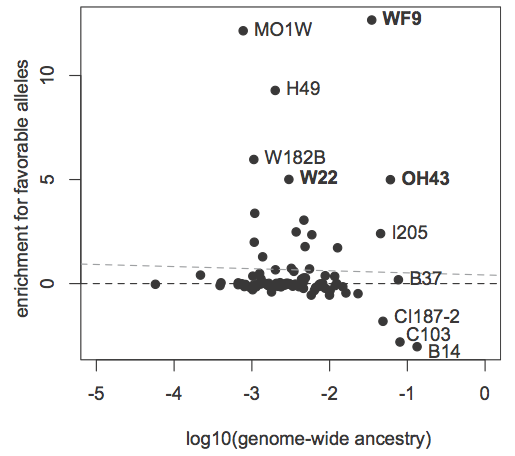
\includegraphics[width=0.5\linewidth]{joost_wf9.png}
\caption{Enrichment (defined as the log probability ratio with respect to control loci) of favorable alleles in older (era 1) inbreds as a function of their average ancestral contribution to modern (era 3) lines. The gray dotted line the regression  with slope −0.1). Inbred names are shown for lines with log probability ratios higher than 4 or ancestry proportion above 0.03. Labels in boldface mark breeding lines of known historic popularity. Figure from \citet{van2012historical}.} 
\label{fig:wf9}
\end{SCfigure}

\subsection*{Lack of public resources limits use of diverse germplasm}

Breeders will not blindly incorporate older material into their populations, however.  
Perhaps the most important piece of information required to effectively utilize older germplasm is pedigree.
Pedigree data immediately gives a breeder information on crosses likely to produce higher yields due to heterosis, and often provides additional utility in identifying likely maturity (flowering time) and other agronomic characteristics. 
Combined with phenotype data, pedigrees can even be used to predict phenotype in the absence of genotype \citep{piepho2008blup} and pedigree-based methods for identifying useful diversity have already been patented by industry \citep{sebastian1995method}.

While private industry may in many cases have detailed records of their own breeding material, the vast majority of private germplasm is founded on $20^{th}$ century public breeding lines \citep{nelson2008molecular}.

Unfortunately, pedigree data for most U.S. maize inbreds is unavailable to most breeders. 
For example, of the over 45,000 worldwide inbreds in the USDA Germplasm Resources Information Network, only some 34,000 have some amount of ancestry determined, and much of this information is incomplete.
If we look at available germplasm only, that number shrinks to 2931 accessions with any available ancestry information.
While there are published compilations of germplasm, these are far from complete:  \citet{gerdes1993compilation}, for example, contains complete pedigree data for less than 20\% of the germplasm in the USDA database.
Moreover, what ancestry information that is available is not in electronic form nor easily accessible in any single resource.  
Instead, historical pedigree information exists primarily in the minutes of breeding committees, old breeding program books, and other hard-copy sources with limited distribution.  

\textbf{We propose to generate an open-source database of public maize pedigrees and use this resource to identify genotypic and phenotypic diversity of high utility in advancing maize breeding.}
Given the importance of maize to U.S. agriculture, this proposal clearly aligns with the USDA AFRI program priorities of ``Plant Breeding for Agricultural Production,'' particularly the ``development and application of tools to predict phenotype from genotype to accelerate breeding of finished varieties''.   
%JRI: Do we include this second quote?  Too long?  Too obvious?  Do we not meet it well enough?
Our proposal will develop tools to accelerate breeding by allowing breeders to more quickly identify useful inbreds, and our application of population and quantitative genetic methods will identify specific genetic and phenotypic diversity of potential use for future breeding.  

\section*{Introduction}
\label{sec:introduction}

%a. Introduction
%Include a clear statement of the long-term goal(s) and supporting objectives of the proposed project. Summarize the body of knowledge or past activities that substantiate the need for the proposed project. Describe ongoing or recently completed activities significant to the proposed project including the work of key project personnel.

\subsection*{Maize breeding}
Maize has undergone dramatic phenotypic and genetic changes since its domestication and subsequent spread across the Americas \citep{daFonseca:2015ey,Doebley:2004ce}. More recently, beginning in the mid-20$^{th}$ century, the intensification of maize breeding efforts has lead to subtler but equally important changes including increasing yields and improved agronomic traits such as leaf angle and density tolerance \citep{duvick2005contribution}. 

Modern breeding programs (post-1960) take advantage of self-fertilization (or now double-haploid technology) to create homozygous inbred lines, which are maintained in separate breeding pools or heterotic groups.
The most important heterotic groups among U.S. public germplasm are the ``stiff stalk'', ``non-stiff stalk'', and ``iodent'' (Figure \ref{fig:diversity}).
Inbred lines from separate breeding pools are then crossed to make hybrid progeny.  
These hybrids often display heterosis, meaning that yield and associated traits of the hybrid are superior to  either inbred parent \citep{Springer:2007bj}.  
Inbreds capable of producing high-yielding, heterotic offspring are said to have good ``combining ability'', and are recycled in their respective breeding pools.
Inbreds that form less desirable combinations are usually discarded from the breeding pool. 
Useful inbreds within a group are crossed with each other, and their segregating progeny evaluated and self-fertilized to create new inbreds. 
Maintaining this system for propagation of inbred lines and hybridizing inbreds for evaluating production traits has worked well for many decades, but there is growing reason for concern that this method may need a genetic boost. 

\subsection*{Decelerating yield gains} 

Maize yields have steadily increased since the advent of hybrid breeding in the 1930's.
But linear increases necessarily mean a decrease in relative gain, and projections suggest that current trends are unlikely to meet future yield goals \citep{grassini2013distinguishing}. 
Of even greater concern is the possibility that the rate of gain may actually be decreasing (Figure \ref{fig:piecewise}).
While some of these yield trends are undoubtedly related to changing management practices, much of the change is indeed due to breeding \citep{Duvick:2001fy}, and current rates of yield gain are lower than historical trends even after correcting for nitrogen fertilizer inputs (data not shown). 

\begin{SCfigure}
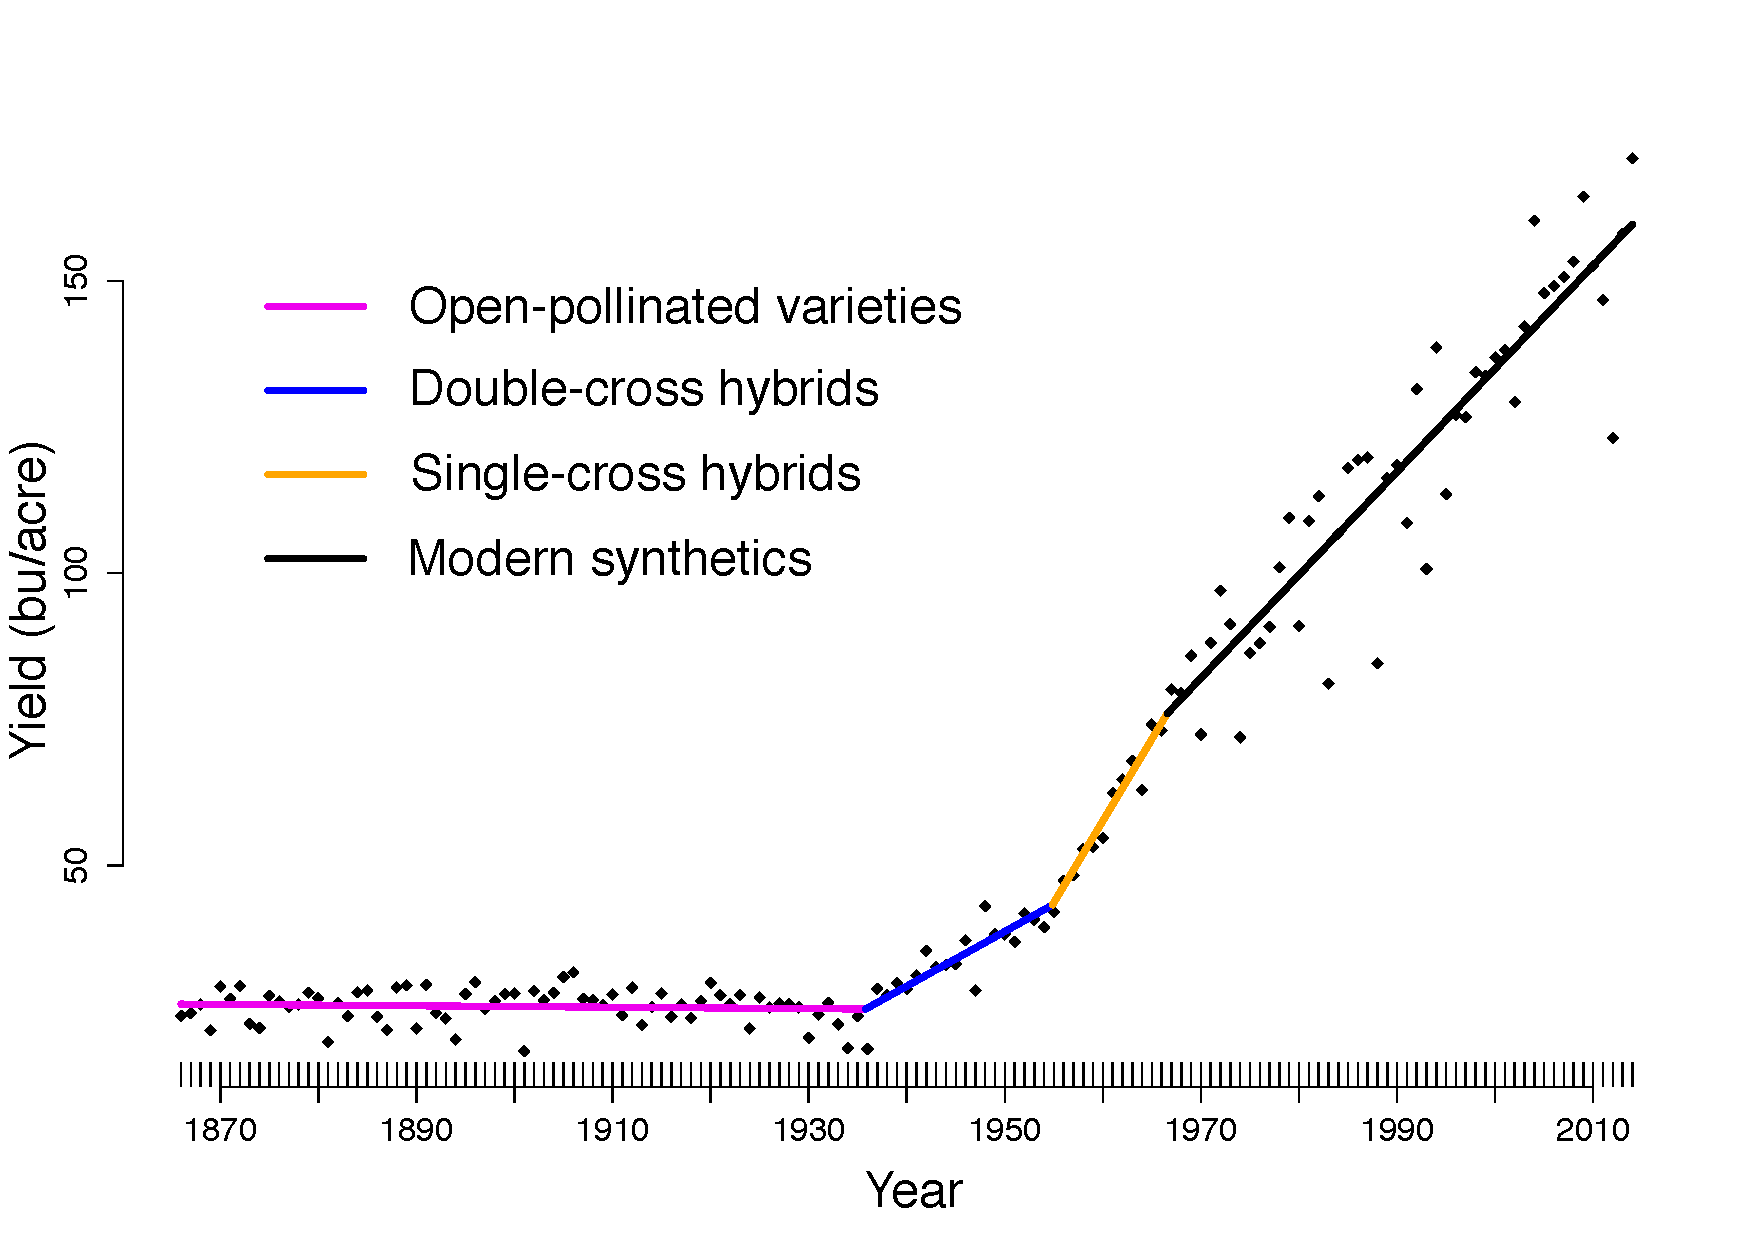
\includegraphics[width=0.6\linewidth]{yield.pdf}
\caption{Piecewise regressions of time against total yield through the four eras of modern maize breeding. Colors represent distinct eras of maize breeding that roughly correspond to the eras  referred to in Figure \ref{fig:diversity}.} 
\label{fig:piecewise}
\end{SCfigure}

\subsection*{Decreasing diversity} 

As selection progresses within a breeding program, inbred lines with poor performance are generally discarded, leading to a decreased effective population size ($N_e$) of the breeding pools.
Response to selection is proportional to the additive genetic variance $V_A$ (equation \ref{eq:lush}), and $V_A$, in turn, depends on $N_e$ as well as the mutational variance per generation ${\sigma}_m^2$ \citep{whitlock1999neutral}:

\begin{align}
E[V_a] = 4N_e {\sigma}_m^2
\label{eq:whitlock}
\end{align}

A reduction in $N_e$ thus inherently leads to a reduced response to  selection, leading to diminishing returns on yield unless new diversity is brought back into breeding pools.
Evidence from the Iowa Reciprocal Recurrent Selection breeding program suggests these concerns are valid (Figure \ref{fig:trends}), as yield gains plateau over time \citep{rouse2003selection} concomitant with continued declines in genetic diversity \citep{Gerke:2013tw}.
Decreasing $N_e$ (Figure \ref{fig:diversity}) in U.S. cornbelt germplasm risks our ability to maintain or increase rates of genetic gain in yield.

%\begin{figure}[ht]
%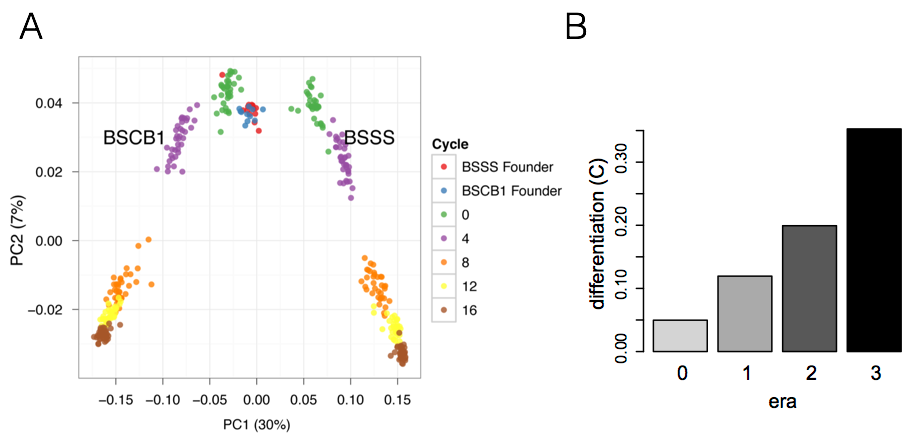
\includegraphics[width=\linewidth]{joostgerke.png}
%\caption{Changes in diversity and population structure during maize breeding.  
%A) Principal component analysis of genotypes from the Iowa Reciprocal Recurrent Selection population. The first eignevector represents divergence between the two heterotic pools, and the second divergence over time within each pool. Figure from \citet{Gerke:2013tw}. 
%B) Population structure --- quantified by the differentiation statistic C --- over time across all U.S. public inbreds. Eras represent time periods in Fig. \ref{fig:diversity}; figure is from \citep{van2012historical} } 
%\label{fig:pca}
%\end{figure}

\subsection*{A novel approach to incorporate new diversity}

Incorporating novel diversity into contemporary modern maize lines is clearly an important goal necessary to maintain and increase rates of yield gain.
While there are other public efforts to achieve this goal, like the GEM  (Germplasm Enhancement of Maize) program \citep{pollak2003history}, these  focus on incorporating exotic germplasm (e.g. CIMMYT lines, tropical hybrids, etc.) into U.S. materials by backcrossing to well-adapted U.S. cornbelt backgrounds.
While this approach is successful at bringing in new diversity, it requires time-consuming back-crossing before it can generate lines that are of sufficient quality to incorporate into a breeding program.

%rjw: this will raise the question --  how the proposed approach will accomplish the desired end result differently, since in the end mining for lost alleles will still require breeding which itself is being presented as the bottleneck here.

%\begin{wrapfigure}{R}{0.5\textwidth}
%\begin{minipage}[t]{0.5\textwidth}
%\begin{SCfigure}
%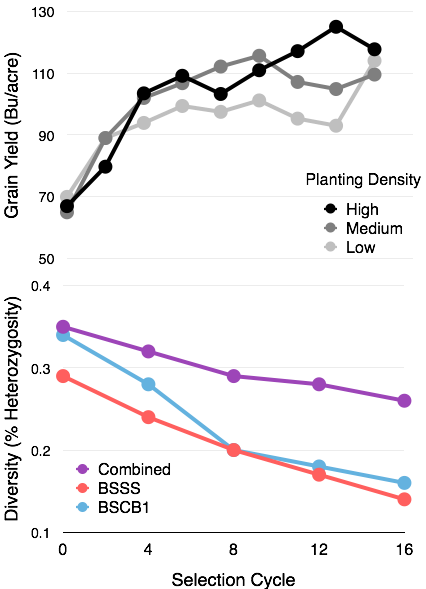
\includegraphics[width=0.5\textwidth]{BSSS.png}
% 
%
%\end{SCfigure}
%\end{minipage}
%\end{wrapfigure}
%\begin{wrapfigure}[30]{R}{0.5\textwidth}
\begin{SCfigure}
    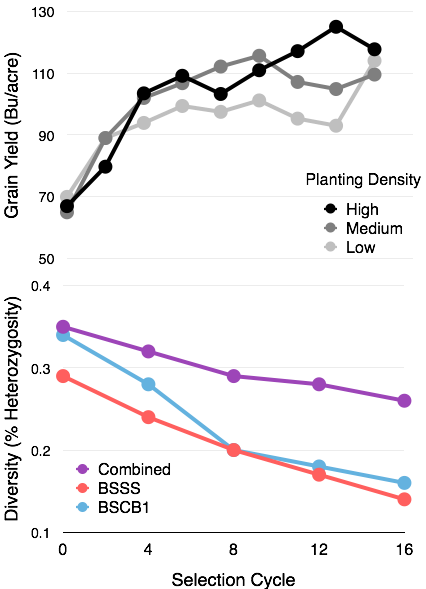
\includegraphics[width=0.4\textwidth]{BSSS.png}
  \caption{Yield and genetic diversity in the Iowa Recriprocal Recurrent Selection Program across 16 cycles of selection. (Top) Grain yield at three planting densities; data are from \citet{rouse2003selection}. (Bottom) Genetic diversity of the BSSS and BSCB1 breeding pools separately and combined; data are from \citet{Gerke:2013tw}.}
\label{fig:trends}
\end{SCfigure}

\textbf{We propose a different approach, using pedigree and genetic data to identify underutilized cornbelt germplasm.}  
While this approach shares with projects like GEM the disadvantage that diverse material is often  agronomically inferior, it has a number of advantages.  
First, in contrast to exotic germplasm, older U.S. germplasm is already reasonably well-adapted to the daylength and climate of the U.S., meaning it can be immediately incorporated into breeding programs without first requiring extensive back-crossing.
Second, with sufficient information (see below), breeders may be able to learn a substantial amount about the potential utility of a line by predicting phenotype directly or understanding its relationship to known material. 
Finally, considerable information is available about many old breeding lines even without prediction, including information on disease 
\textcolor{red}{MORE ADVANTAGES??}

\subsection*{Identifying useful diversity}
As any breeder will attest, many old lines have fallen out of use precisely because they showed inferior agronomic performance under a particular selective regime (drought, disease resistance, etc).
There are a number of reasons, however, why older lines may retain useful genetic diversity.
First, lines are often discarded or selected against because of poor performance for a particular trait, which does not preclude that line's utility in breeding for other traits.
For example, thanks to its combining ability, the U.S. inbred B73 quickly spread in popularity and now makes up a considerable portion of modern breeding material \citep{van2012historical}. 
Yet when evaluated for drought and heat stress, B73 significantly underperformed compared to less well-utilized lines such as B76 \citep{chen2012characterization}.
Second, the contribution of older lines to modern germplasm does not necessarily reflect their genetic potential.
Our analyses of maize ancestry found popular lines with fewer beneficial alleles than expected given their importance to modern germplasm as well as lines with more beneficial (as defined by a steady increase in allele frequency over time) alleles than expected (Figure \ref{fig:wf9}).

\jri{blah blah blah blah


 popgen point about alleles lost due to drift
 previous efforts like our popgen only looked at allele frequency. this is problematic because of structure etc.
 pedigree analysis allows improved popgen and other benefits (discuss)}
 

\subsection*{Pedigree-based approaches to identifying useful maize germplasm}


\subsubsection*{Advantage of pedigree vs. disadvantages of other approaches}
Most release sheets and information in NPGS on modern inbreds contain not only parentage information, but a wealth of important phenotypic information and the selective regime used in propagating a given line. 
As an example, a regular expression ``grep", case-insensitive search for counts of character strings of terms that might typically be associated with selection regimes  (Figure \ref{fig:words}), such as ``resistance'', ``tolerance'', ``blight'', ``drought'', ``disease'', etc - reveal that indeed, many lines with ancestry information were targeted by breeder's for different phenotypes. 
If 
Broadly, most inbred lines have been selected for ``combining ability'' across the pedigree, but other programs are more targeted in their choice of selective regime: blight resistance, maize mosaic virus, drought resistance, etc. 

\begin{figure}[t]
        \centering
        \begin{subfigure}[b]{0.5\textwidth}
                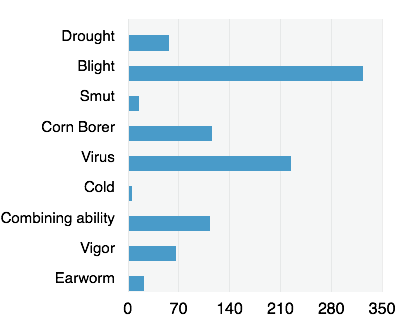
\includegraphics[width=\textwidth]{disease.png}
                \caption{}
                \label{fig:words}
        \end{subfigure}%
        ~ %add desired spacing between images, e. g. ~, \quad, \qquad, \hfill etc.
          %(or a blank line to force the subfigure onto a new line)
        \begin{subfigure}[b]{0.5\textwidth}
                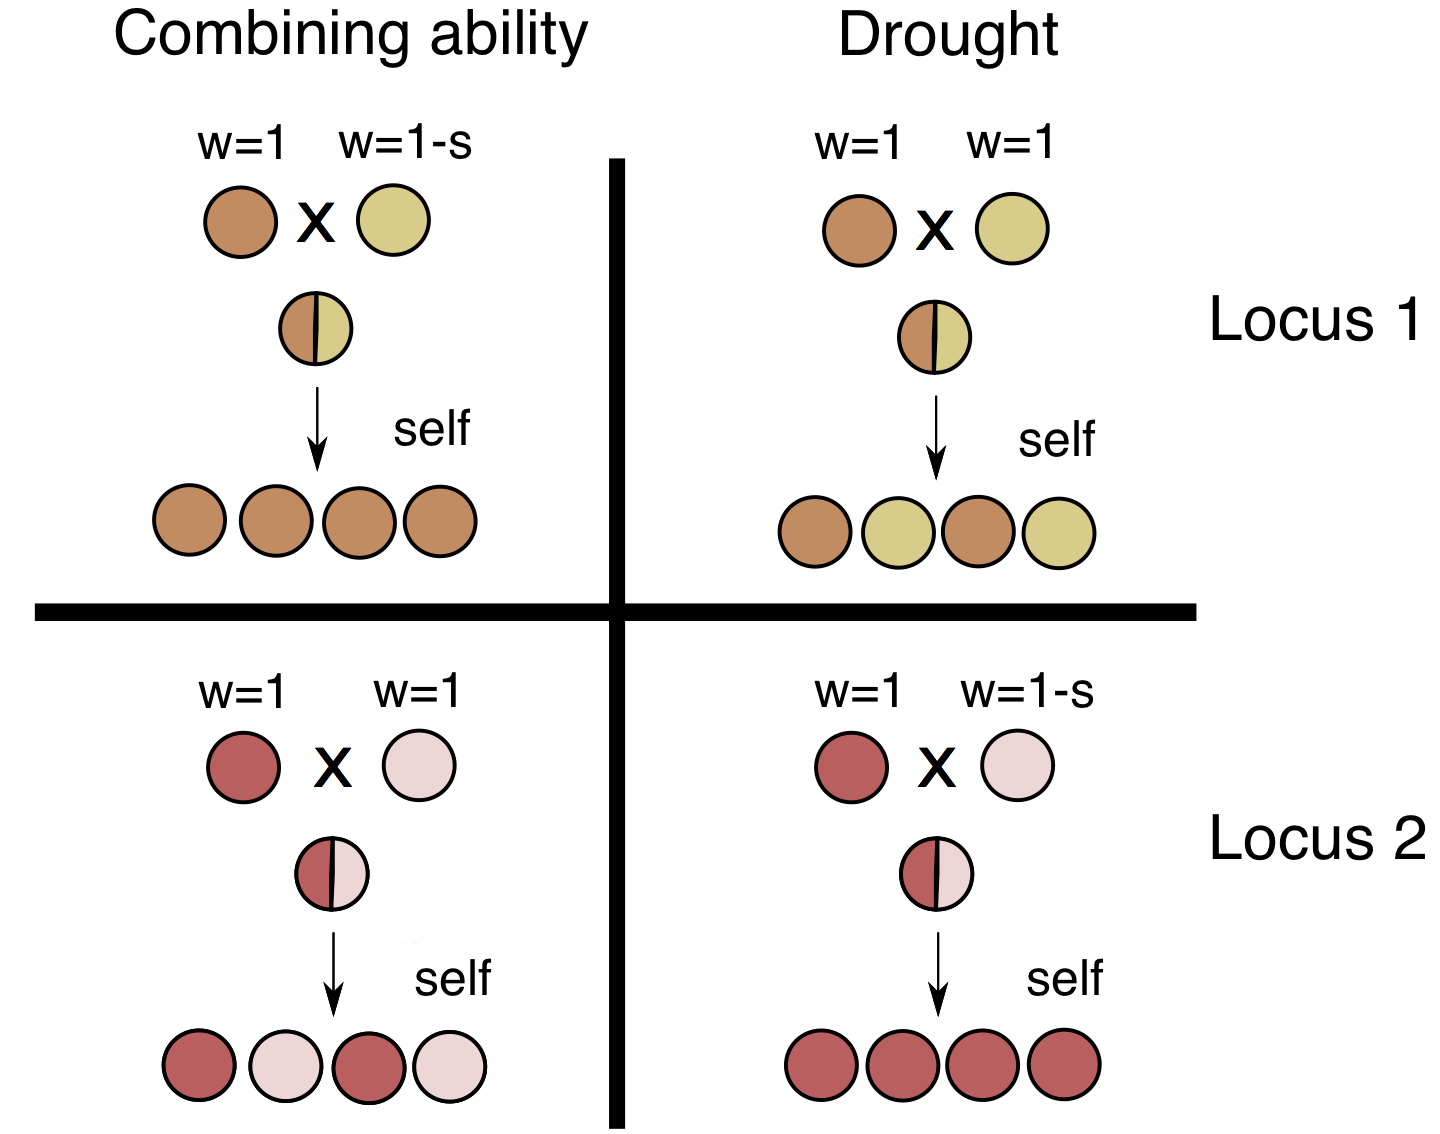
\includegraphics[width=\textwidth]{divergent.png}
                \caption{}
                \label{fig:div}
        \end{subfigure}
\caption{\textbf{a)} Counts of a small set of germplasm descriptors from the USDA database. \textbf{b)} Expected segregation of alleles at loci for two traits in different breeding programs.  Selective regime for combining ability across two example breeding programs and loci. Fitness (w) of each allele indicated, with selection coefficient (1-\textit{s}) for the allele being selected against in a given regime. Locus 2, though beneficial under drought conditions, risks loss due to drift in breeding programs focusing only on combining ability. }
\end{figure}

Using expectations of relatedness coefficients between \textbf{known} close relatives (inbred parents-inbred progeny) we can compare to observations of genomic sharing, where significant deviations from expected relatedness coefficients would tend to indicate selection. 
Across the entire pedigree, we expect that certain alleles will go to fixation due to breeder's selection as they are beneficial for ``combining ability''. 
But, within smaller breeding programs (and pedigrees) under a specific selective regime we will observe only 



\begin{itemize}
\item observed vs. expected allow us to look allele specific ``hard'' breeder sweeps across the pedigree for combining ability
\item but phenotypic information of each program contained in release sheets may also allow us to look at selective regimes within programs (while selection is relaxed in others).
\item If alleles exist in other programs along with the specific diversity of that program, we can target those.
\end{itemize}



\subsubsection*{Preliminary work: pedigree records to date}
To date, we (Drs. Smith and Crosby) have gathered parentage info for over 3193 lines and originally built a large pedigree of some 700 lines (Figure \ref{fig:b73isbig}is but a small portion of this pedigree) with complete parentage information that overlaps with currently available GBS maize 2.7 data \citep{Glaubitz:2014eu}. 
Currently, we have a total of 1696 unique (1900 duplicate) records overlapping with GBS data, which is stored in a rudimentary SQL database. 
These records can be queried based on unique identifiers from the USDA (PI numbering system) or based on its ``classic inbred line name'' that most breeders recognize.


\subsubsection*{Preliminary work: allele dropping works? GBS pruning?}


\begin{figure}[ht]

\includegraphics[width=1.0\linewidth]{pedigree_poster.pdf}
\caption{Reconstructed pedigree data for the inbred line B73 that features heavily in modern germplasm.}
\label{fig:b73isbig}
\end{figure}

\paragraph{unincorporated text $->$}
Pedigrees, especially when combined with modern genomic and phenotypic trait data, are useful tools for predicting phenotype \citep{crossa2010prediction} and identifying beneficial alleles \citep{sebastian1995method}.
 that have experienced strong artificial selection across breeding pools. Examples of their application can be found with: cattle \citep{Decker:2012kd}, soybean (cite), and grape (cite). 
While private companies likely have their own pedigree databases to do exactly this, these data are private, patented, and not available to the public. 
Further, much of the pedigree information on older founder inbred maize lines sits in old volumes of Crop Science or the Agronomy Journal, experimental station technical bulletins, regional corn breeding meeting records, release sheets, or breeding books, unused and vulnerable to loss.  
The National Plant Germplasm Service (NPGS) database contains information with regards to ancestry of public maize inbred lines, much of this information is incomplete or missing (see section above). 
However, much of this ancestry information on modern maize lines  is still publicly available, only not in digital form, nor is it easily-accessible. This historical pedigree information exists in old volumes and minutes of breeding committees, old breeding program books, and other hard-copy-only sources. Here, we propose a project that will help preserve, maintain, and use this historical information with novel genomic data to better benefit future maize breeding programs.

\section*{Approach}
\label{sec:approach}
Our proposed research has three major aims in using pedigree information to detect historic shifts in allele frequencies of modern inbred maize lines.

\begin{itemize}
\item Aim 1: Digitize and curate pedigree and genotype information into a publicly available database. 
\item Aim 2: Identify useful diversity using a combination of pedigree and population genetic approaches.
\item Aim 3: Phenotypic and genotypic evaluation of individuals lines that feature heavily in the historical pedigree.
\end{itemize}

\subsection*{Aim 1: Public pedigree curation}
Our first aim is  stop the potential loss of hard copy pedigree data by gathering it from land grant institutions that previously hosted breeding research programs of maize inbred lines. 
We have good reason to believe this information that could help complete the public pedigree is likely archived in their libraries . 
The land grant schools of importance were identified by two maize breeding experts named on this grant: Dr. William Tracy and Dr. Oscar ``Howie'' Smith who have between them +70 years of breeding experience in maize. 
Dr. Tracy was a co-author on the leading pedigree book on maize lines \cite{gerdes1993compilation} and Dr. Smith spent 7 years as maize breeder for the USDA, and then a further 20+ years working as a maize breeder for Dupont Pioneer.

The land grant schools they have identified include: the University of Wisconsin, Virginia Tech, the University of Georgia, the University of Florida, Pennsylvania State University, the University of Nebraska, North Carolina State University, the USDA station at the University of Missouri. 
Dr. Tracy (based at the University of Wisconsin) and Dr. Holland's student (based at North Carolina State) will largely be responsible for visiting these schools in the first year to obtain and digitally scan this information with portable digital scanners. 
Dr. Randall Wisser's student will be responsible for visiting two schools starting in the second year of the grant.
Dr. Tracy will obtain information from the University of Wisconsin (host institution), the University of Florida, and the University of Nebraska. 
Dr. Holland's student (in the first year) will be responsible for North Carolina State University (host institution), the University of Georgia, and finally, the USDA station at the University of Missouri. 
Dr. Randall Wisser's student (to start in year two of the grant) will be responsible for the University of Pennsylvania and Virginia Tech.
Drs. Tracy and Smith have extensive contacts with faculty past and present at these schools, so obtaining the information and scanning it at each school traveled to should take no more than a few days. 

Dr. Kate Crosby, Dr. Taner Sen (support letter from maize GDB enclosed), senior personnel Dr. Oscar Smith, and CO-PI Dr. Bill Tracy will consult on an agreed upon standard format with which to store the raw scan of pedigree records, the phenotypic and genomic information. 
Establishing an agreed upon format in the first few months before the scans are obtained will enable easy mapping of current and future genomic data formats to pedigree information.

We fully anticipate that we will isolate some lines that feature heavily in the historical pedigree and have germplasm available, but that do not have any genomic data available for them. 
In such cases (where germplasm is available), we intend to use genotype-by-sequencing (GBS) \citep{Elshire:2011ha} as a cost-efficient platform \citep{Glaubitz:2014eu} to obtain high-coverage and density of SNPs  for these lines, with markers aligned to the newest maize reference genome (currently B73 v. 3). We anticipate that this number of lines should be no more than a few hundred samples of inbred lines, or two-four plates worth of samples (192-384 inbred lines).
In addition to serving as contact for obtaining hard-copy breeding information, Dr. Sherry Flint-Garcia will serve as a contact at the USDA station to help Dr. Holland's student understand how inbred lines are deposited, uniquely named, and will also be able to help the student obtain any available USDA germplasm deemed to be important in the pedigree, but not yet genotyped.

\subsubsection*{Expected outcomes (Aim 1)}
Our main deliverable from the first aim is an \textbf{open public pedigree database to be hosted on maize GDB (http://www.maizegdb.org/) for the long term future.} Users will be able to contribute and revise incomplete information, with the goal of establishing a nearly complete public pedigree of maize inbred lines. \textbf{To our knowledge, this will be one of the first public crop databases of its kind (with lines having genomic and phenotypic data mapped onto entries).}  

The initial database will house information on release dates, selection regime, historical phenotype information, germplasm availability (or nearest neighbor germplasm availability).
Breeders and researchers will be able to query information on lines across many years, their closest relatives, and additionally for alleles that are associated with a given a selection regime. 
For instance, if a breeder wants to establish an inbred line that is both drought and blight resistant, they could query information on lines that are drought resistant and lines that are blight resistant, plus query how other alleles in a chosen line might be associated with other traits of interest. They could then decide on crosses and breeding designs in the field, and update information (should they choose) on maize GDB following actual growouts.
\kc{include this or ditch? Additionally, Dr. Kate Crosby is currently investigating the possibility of using no-SQL database without formal schemas specified \textit{a priori} (graph databases) to be able handle queries with respect to mapped genomic data, extended ancestry, and phenotypic data, along with new visualization tools \citep{ParejaTobes:2015bf}.}
Ensuring data, code, and script are open-access or open-source (freely available to the public) is important for critique, debate, and dialogue in science. Dr. Ross-Ibarra has a long track record of ensuring openness with his science, data, and code. Throughout this project, both Dr. Ross-Ibarra and Dr. Crosby will endeavour to ensure that code and data are available via repositories such as github, figshare, maize GDB, and iPlant.



\subsubsection*{Potential pitfalls \& limitations (Aim 1)}
While we are very optimistic about the prospect of obtaining accurate pedigree information from these various institutions the nature of corn-breeding and record keeping of corn-breeding can be nebulous. 
Ideally, we would be able to accurately count the number of meioses in the total pedigree, in each breeding program, down to each line; thus, retracing the complete ancestry of a given contemporary inbred. 

However, in many cases, it may not have been noted at which point in a breeding program a line was bulked at, nor on occasion which lines were used in recycling an inbred when seed was exhausted. 

For instance, a record from NPGS may indicate that a line was bulked and stored after being selfed to generation 6, or it may have been bulked and stored following selfing at generation 4. As a ballpark figure, a ``selfed generation 6 inbred'' means that germplasm from that line is 99\% homozygous at all locus pairs. 
Meaning that if this inbred is selfed further, not much changes with respect to levels of homozygosity nor heterozygosity (as recombination via selfing is ineffective beyond this point).  
Thus, so long as an inbred is at or beyond cycle 6, it will be kept, but inbreds before this period shall be discarded.

To ensure that historical records of inbred lines are isolated following the sixth generation of selfing and beyond we will investigate the level of heterozygosity in each of these lines with GBS data relative to the total amount of missing data in an individual line. 
Within reasonable confidence limits most lines should show a very small portion of heterozygous loci even with GBS markers (known to have a high rate of error in the under-calling heterozygous). 
Historical pedigree records and other information on old lines may be available, but the germplasm from these old lines may simply not be available (genomic data will not be able to be mapped onto these lines. 
Currently, we know that approximately 12.9\% of germplasm from NPGS for which we have parentage information is not available. 
Undoubtedly, as we add more records from breeding books, journals, meeting minutes, and research station bulletins, we expect a similar level of unavailability of germplasm.  
In such cases, we would seek available germplasm from the next nearest relatives according to historical information, and genotype those accessions. 

\subsection*{Aim 2: Identify useful diversity}

\subsubsection*{Mendelian segregation on a pedigree}
As different lines have been under different historical selective regimes or breeding programs, these phenotypes likely have an underlying genetic basis. Following the digitization of historical information, the Dr. Holland's student and the post-doc (Kate Crosby) will construct many small pedigrees of the different selection regimes and use the technique of \textbf{``allele-dropping''} to further identify breeder's selection and useful diversity. 

``Allele-dropping'' is a patented method \cite{sebastian1995method}, used in industry and works by identifying distorted segregation at all heterozygous loci within a single pedigree/breeding programs and across many pedigrees/breeding programs (Figure \ref{fig:alleledrop}). 
As a simple Mendelian approach this technique identifies traces of selection by directly accounting for ancestry, and without the worry of having to account for shared population structure \cite{sebastian1995method} (as can often be a problem or limitation in modern population genomics approaches). 

If we observe the uni-directional shift of a given allele across many of these small pedigrees at a set of loci (or even within just one pedigree in a specific breeding program), this would tend to indicate selection. 
We would tend to predict that a consistent subset of alleles that are associated with combining ability would tend to increase in frequency across the pedigree.
As an example, using Mendelian rules and starting with a mostly homozygous line (with some residual heterozygosity), we can examine single heterozygous locus (i.e. $Aa$). 
Because we know what our expectations ($E$) for number ($N$) of $AA$ (or $aa$) homozygous inbred progeny at generation 6 (under no selection) should be (given by $E = 1/2 N$), we can compare to the actual observed number of progeny. 
If our observations deviate from this expectation, we would tend to conclude breeder's selection for these alleles (especially if observed across a good portion of the entire pedigree). 

\begin{figure}
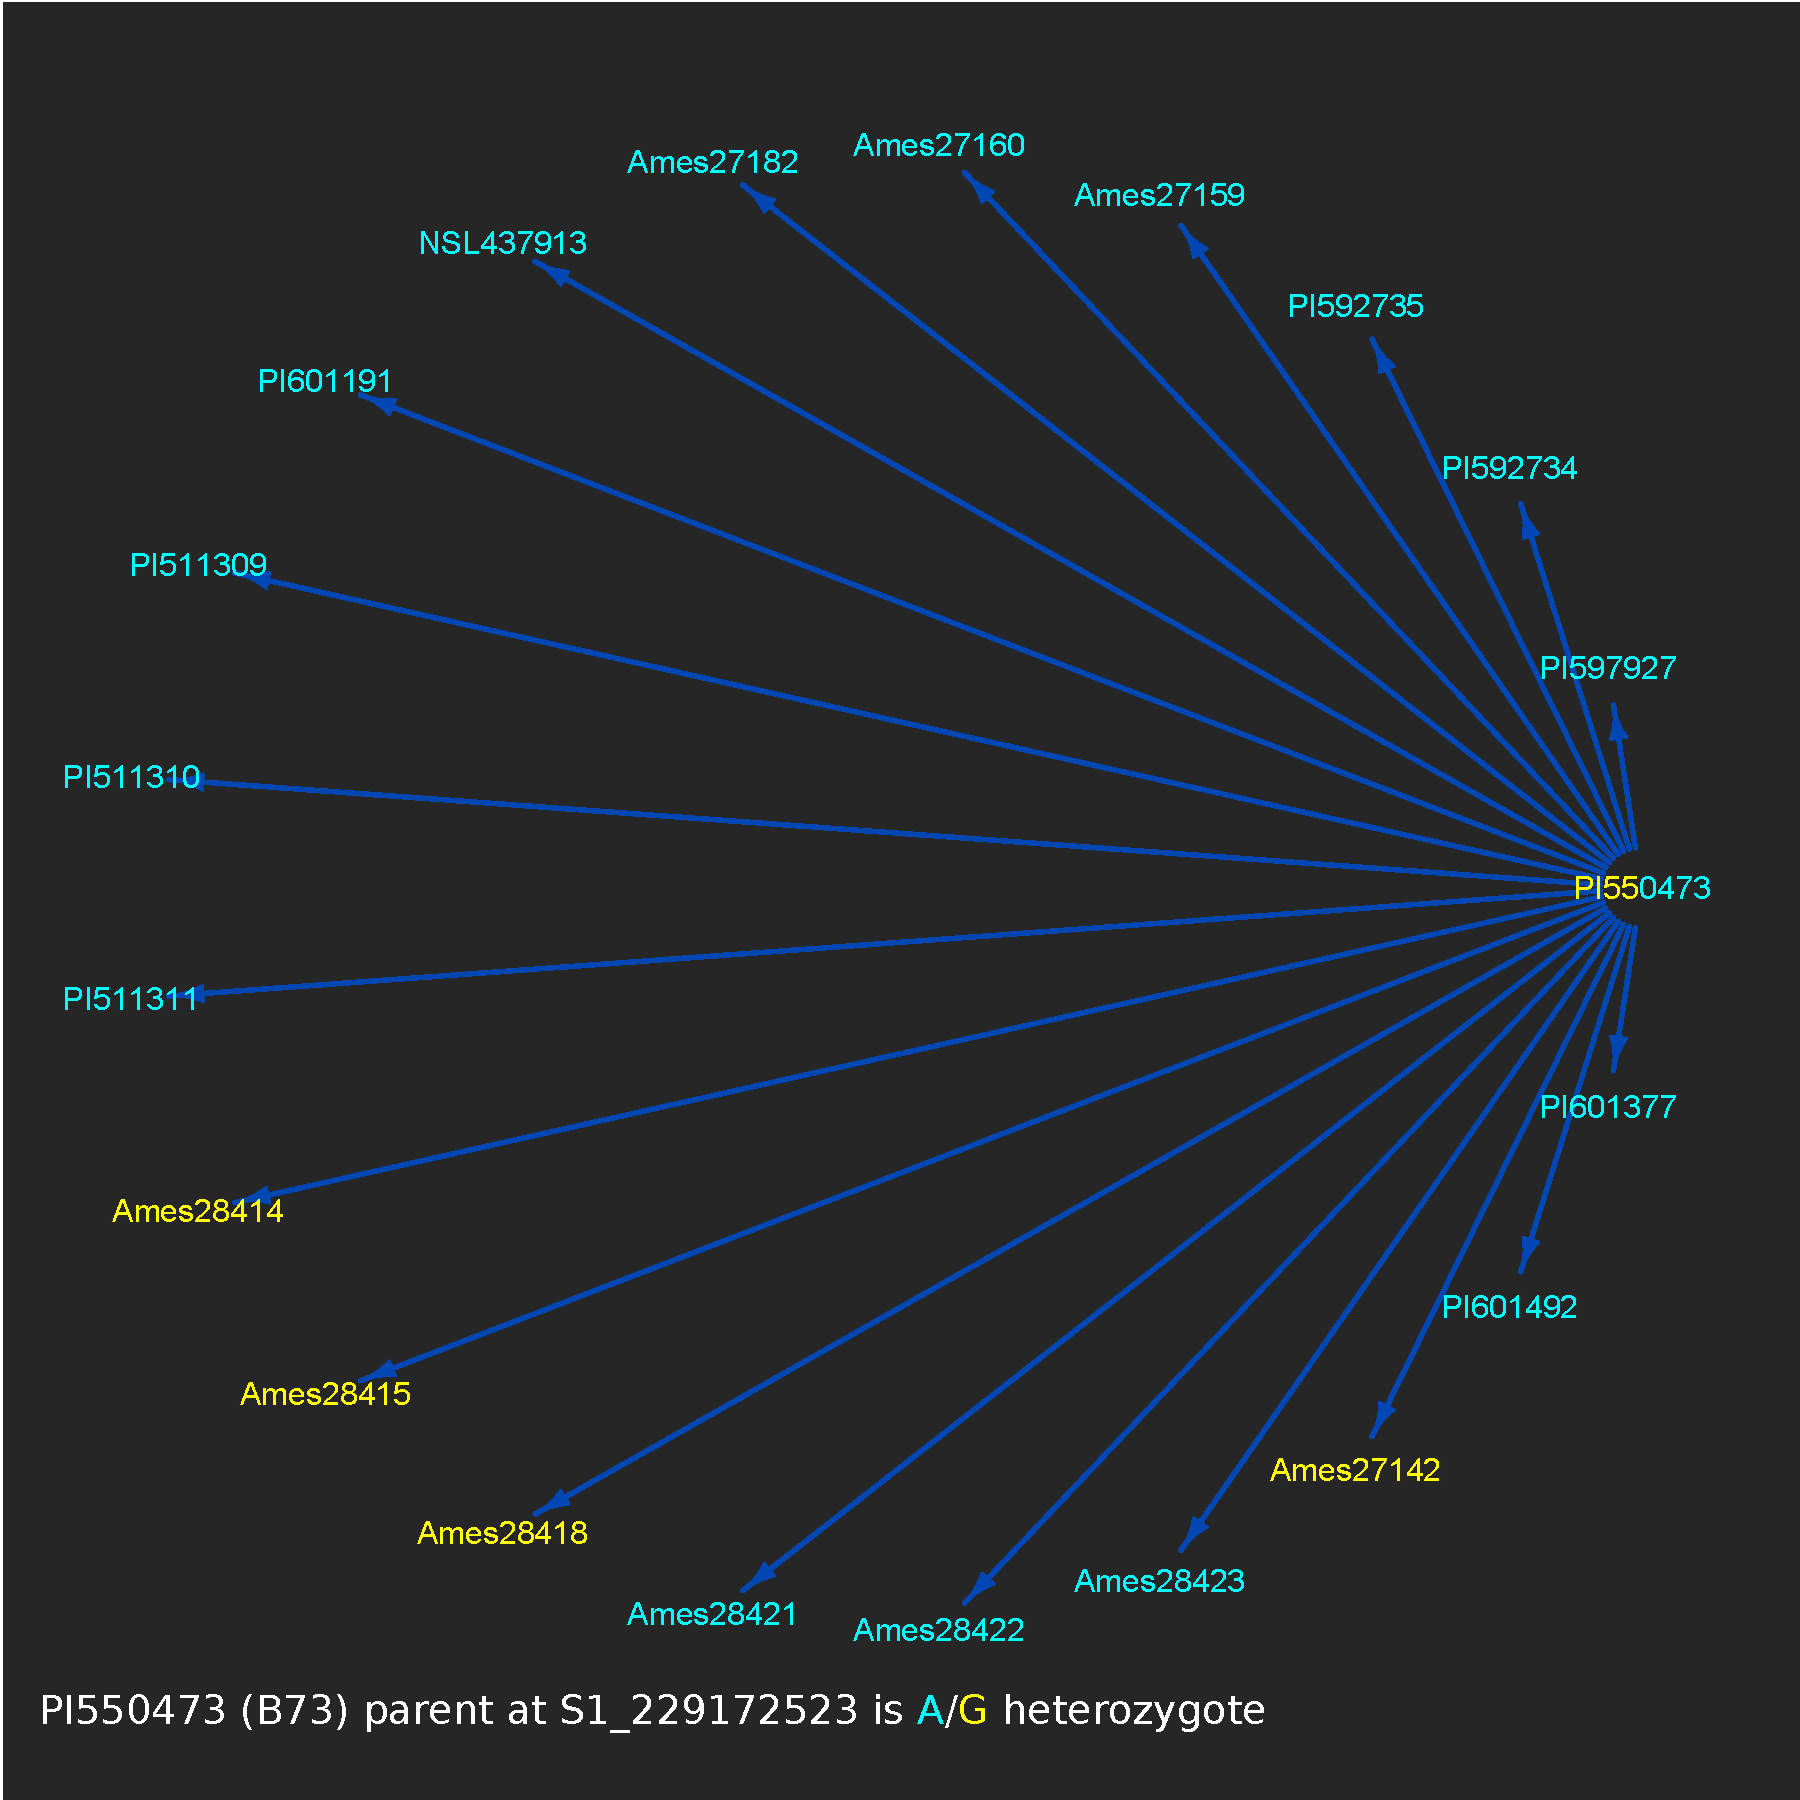
\includegraphics[width=0.5\linewidth]{Pruned.pdf}
\caption{B73 (also known as PI550473 by NPGS and a number of its inbred progeny) is heterozygous at 379 loci out of over 954,000 loci with GBS markers). The blue labels represent which inbred progeny obtained the A allele, whereas the yellow labels indicate the progeny that have obtained the G allele at a particular locus. \textbf{NB: the other parent of these lines is not indicated for simplicity}.}
\label{fig:alleledrop}
\end{figure}

Our current preliminary data set of 1696 accessions contains a fair amount of information on different selection regimes (Figure \ref{fig:words}). 
By applying allele-dropping to a number of these smaller breeding programs, and tracking unidirectional shifts, we (Dr. Holland's student and Dr. Crosby) will attempt isolate strong signals of breeders selection for a given selective agent (within a program). 
We may then look for these alleles across all other breeding programs where selection was presumably relaxed (Figure \ref{fig:div}), and if we can isolate these alleles, then they may be introgressed back in as useful diversity to other breeding programs.

\subsubsection*{Potential pitfalls \& limitations (allele-dropping)}
One of the potential limitations with the allele-dropping approach is that we may lack the statistical power to detect selection on individual alleles, because there may be too few progeny of each line under a given selection regime. 
However, this limitation of power is not an issue for the complementary population genetic approach we plan on using: the $Q_{x}$ method described in \cite{Berg:2014bs}. 

\subsubsection*{Predictive phenotyping ($Q_{x}$)}
\jri{here we show that if individual lines predictive phenotype is better than expected given pedigree/genomic background, then it's likely a good choice for breeding! }
Genotypes when combined with a pedigree can be used to predict phenotypes \citep{de2009predicting,crossa2010prediction,Decker:2012kd}.  
By using allele dropping we target individual loci within and across breeding programs. But, allele dropping may not have the statistical power to detect a more diffuse polygenic signal of adaptation. 
Significant hits from a genome wide association study (GWAS)  can be summarized as the allelic effects $\alpha^{2}$ (or breeding values) that breeders can take advantage to get an estimate of $V_{A}$ for any trait of interest. $V_{A}$ can be estimated for one locus (equation 1 below) or summarized across all loci $L$ in the genome (equation 2 below):

  \begin{align}
    V_A = 2pq\alpha^2
 % \end{equation}\break
 % \begin{equation}
    V_A = \overset{L}{\underset{l=1}{\sum}}\alpha^2_l2p_l(1-p_l)
  \end{align}

If alleles are at high frequency in certain breeding programs and can also associated with a beneficial phenotype (e.g. blight resistance), they are potentially beneficial alleles that could be resurrected and introgressed back into a modern breeding program. 
By then searching the entire pedigree for these alleles and isolating those lines that have these SNPs, they may be targeted by breeders and public research programs.
Further, the greater the $V_A$ of a trait (the greater the allelic diversity of that trait, i.e. $N_{e}$), and thus, the greater $R$ (response to selection) to any new selective program a breeder chooses to apply.


\subsubsection*{Expected outcomes (Aim 2)}
We will identify alleles useful for breeding using several approaches, first
\begin{itemize}
	\item compare GWAS SNPs to allele dropping (may lack power) - mention Holland's student
	\item use GWAS SNPs to also do Qx (complementary approach where power is less of an issue) within and across pedigrees
	\item ideally every single method used will isolate a consistent set of SNPs, these we would have a very high confidence that they are under selection
\end{itemize}

\jri{identification of lines with good alleles. identification of new phenotpyes undergoing selection? for pitfalls perhaps lack power for individual alleles, but this is complemented by the Qx approach.}



\subsection*{Aim 3: Field testing individual lines}
\jri{explain we don't have feasibility of doing large scale testing, but this is meant as a proof-of-principle to ground-truth our strategy. }
In order to test the idea that phenotypes

%\jri{year 2 plot we grow up stuff that we want phenotypes and genotypes for}

%\jri{year 3 plot we grow up 50 bad lines, 50 good lines (steal the design from my email, 2 rows of 10 each, phenotype middle 5, what traits, etc. to compare predicted "good" lines and predicted "bad" lines.  We also include as checksd some set of ex-PVP -- see my email to Randy for details}

\subsubsection*{Expected outcomes and potential pitfalls: Aim 3}
%\jri{year 2 fills in important gaps in pedigree data and genotyping. year 3 tests our predictions. explain it will not be comprehensive, but should give an idea of how well things work, as well as an idea of the agronomics of the old lines -- if even the "best" old lines have terrible agronomics, we'll know our whole idea is probably not great.


Should loci be identified as having uni-directionally shifted through time across many of these small pedigrees, we would compare this to our findings in project 2 (see next section \textbf{project 2}).


\subsubsection*{Project 2 for student 2: novel population genomics approaches to project current phenotypes back in time}
%Probably should explain Qst and Fst more? Latta's intro is clear on this problem.

%-Do I provide Qx statistic here?
Dr. Randall Wisser's student will be responsible for performing this analysis on lines deemed to be of interest from both periods (likely those founder parents and their progeny or later generation ancestors). 
%I know Qx accounts for structure - but I think looking at inter-familial and extra-familial will be cool (different covariance matrices for sure.
The student will then grow out these lines as a way of verifying that the SNPs in earlier founder lines shared with later familial and extra-familial lines express the expected additive phenotype for production traits of interest. 
By combining population genetics with quantitative 



\subsection*{Expected outcomes \& Utility of results}


\subsubsection*{From quantitative genetics to population genetics and back again}



\subsection*{Means of analysis/interpretation}
Dr. Randall Wisser has agreed to provide plot space for growing up germplasm of lines disproportionately present in the pedigree that have phenotypic data affiliated with their release sheets or with NPGS, i.e. drought resistance, heavy-metal tolerance, disease resistance, etc (see attached facilities sheet at the University of Delaware). 
The main purpose of this grow-out is to ground truth both the information from release sheets and compare this to the suppositions gained from \citep{Berg:2014bs}, with lines that appear to harbor alleles that contribute to production traits (see section above).


\subsection*{Timeline}
A graphical timeline of our three-year proposal is presented below. %Holding back till hear from Holland

The first year will be spent traveling and gathering and digitizing pedigree records at land-grant institutions.
Dr. William Tracy and Dr. James Holland's masters student will largely be responsible for traveling to and scanning hard-copy records into digital format. Dr. William Tracy has committed to obtaining records from the University of Wisconsin, University of Nebraska, and will also visit the University of Florida. 
Dr. James Holland's student will be responsible for the breeding records at North Carolina State University, Virgina Tech, and the inbred records housed at the USDA at the University of Missouri. We estimate that this should take no longer than a few weeks at each institution with the first student or CO-PI. 

%\jri{timeline needs to be brief and say what's happening when. stuff like this goes up above in the how.}
The scanned digital records must then be translated into a usable data format for further analysis with NGS or phenotype data. At worst, this will involve the student, CO-PI (Holland or Tracy) or the postdoc (Crosby), physically reading and translating each of the scanned papers, and this could take several months to the entire first year depending on volume of records. 
Dr. Kate Crosby with assistance from Dr. Oscar Smith, Dr. William Tracy, with cooperation from Dr. Taner Zen will be responsible for ensuring a consistent data format for hosting on maize GDB.

At the start of the second year, any inbred line that is disproportionately present in the pedigree with available germplasm, but that has no to little genetic information on it will be genotyped using the GBS platform. 

Dr. Randall Wisser's student will then start and over a period of 3-6 months will learn the population genomics approach presented in \citep{Berg:2014bs}, as well as identify and incorporate phenotypic information into the database from the data gathered in year one. 
As a way of ground-truthing the phenotypic data and assessing the , Dr. Randall Wisser and his student will grow out lines deemed to have favorable production traits.

\newpage
\bibliography{kc.bib,jri.bib}
\end{document}